% Author: Till Tantau
% Source: The PGF/TikZ manual
\documentclass{article}

\usepackage{tikz}
\usetikzlibrary{mindmap,trees}
\usepackage{verbatim}

\title{Genomics Notes}
\date{12 Nov 2021}

\pagenumbering{arabic}

\begin{document}
	\pagestyle{empty}
	\maketitle
	
	\tableofcontents
	
	\newpage
	\section{Overview}
	
	The mind map gives the concepts that are outlined later on in the document
	
	
	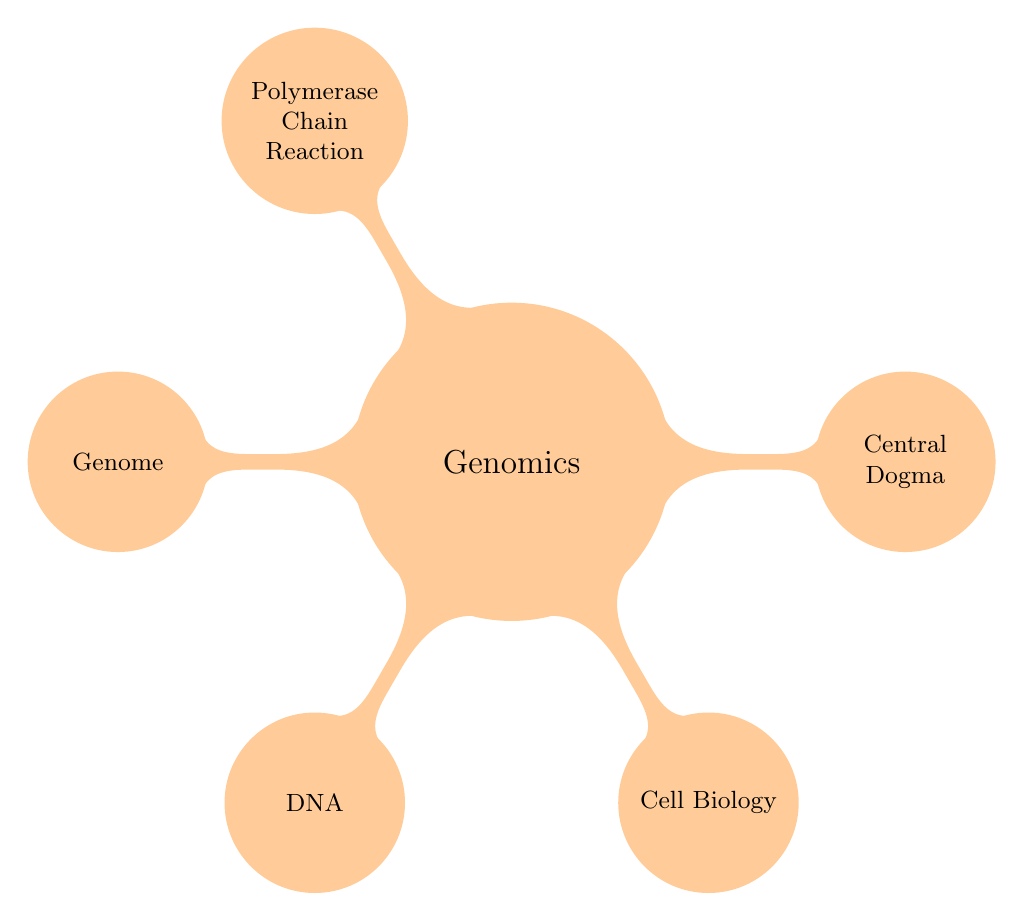
\begin{tikzpicture}[mindmap, grow cyclic,clockwise from=0, every node/.style=concept, concept color=orange!40, 
		]
		\node{Genomics}
		child { node { Central Dogma}}
		child { node { Cell Biology }}
		child { node { DNA }}
		child { node { Genome }}
		child { node { Polymerase Chain Reaction}}	
		;
	\end{tikzpicture}

	\section{Central Dogma}
	\begin{itemize}
		\item DNA gets transcripted to RNA
		\item RNA gets translated to protiens
	\end{itemize}

	\section{Cell Biology}
	\begin{itemize}
		\item Eukaryotes : cells with nucleus. DNA is in the nucleus
		\item Prokaryotes : cells without nucleus
		\item Diploid: two copies of every chromosome, and then X,Y chromosomes
		\item Mitosis: process of cell dividing into 2 cells
		\item Meiosis: crossing over of chromosomes from the father and mother to create child's chromosome
	\end{itemize}
	
	\section{DNA}
		\begin{itemize}
			\item Chromosomes are DNA molecues glued by something called histone
			\item DNA has the genetic material passed on from generations
			\item Adenine and Guanine are prunies with two ring structure
			\item Thymine and Cytosine are pyrimidines, with single ring
			\item In double helix structure, A binds to T and G binds to C
			\item A,G,T,C are called nucleotides
			\item RNA is single strand and Thymine is replaced by Uracil
			\item Three RNA nucleotides get translated to one protien amino acid
		\end{itemize}
	
	\section{Genome}
	\begin{itemize}
		\item All the nucleotide sequences including Exons and Introns
		\item Exons are DNA sequenes that get transcripted to RNA
		\item Introns are skipped during RNA making
		\item Introns can have tandem repeats
		\item Genotype is collection of sequence of genes
		\item Phenotype is observed trait
	\end{itemize}

	\section{Ploymerase Chain Reaction}
	\begin{itemize}
		\item A way to make many copies of DNA
		\item Suppose there is a strand of DNA we want to replicate
		\item The beginning and end of that sequence, we take a primer molecule which is a few bases long
		\item Then there are lot of nucleotides put in the mixture
		\item And then there is DNA polymerase molecule
		\item The mixture is first heated and then DNA strands gets seperated
		Then mixture is allowed to cool and then primers attach themsleves to these strands
		Primers are the complement of the starnd beginning and end we want to replicate
		Then the DNA polymerase looks at the DNA that has incomplete double strand - which will be in between the places where the primers got attached
		The DNA polymerase will take the floating nucleotides and bind it to single strand and complete the DNA seqeunce
		The cycle is repeated, each cycle the aount doubles
	\end{itemize}
	
\end{document}